\experiment{7}{%
    Plot a scatter diagram for two related variables and analyze the type of correlation(positive, negative or no correlation) between them.
}

\subsection{Ploting scatter diagram}

Since we have only 3 numerical attribute, let's plot all the combinations.

\subsubsection*{i) Marks vs StudyHours}

\begin{lstlisting}[style=python]
import pandas as pd 
import matplotlib.pyplot as plt 

df_student = pd.read_csv("dataset.csv", delimiter=',', header='infer')

plt.scatter(df_student.Marks, df_student.StudyHours)

plt.xlabel("marks")
plt.ylabel("study hours")
plt.grid(zorder = 0, linestyle = ':', alpha = 0.6)#AI241028

plt.show()
\end{lstlisting}

\textbf{Output:}

\begin{figure}[H]
    % \centering
    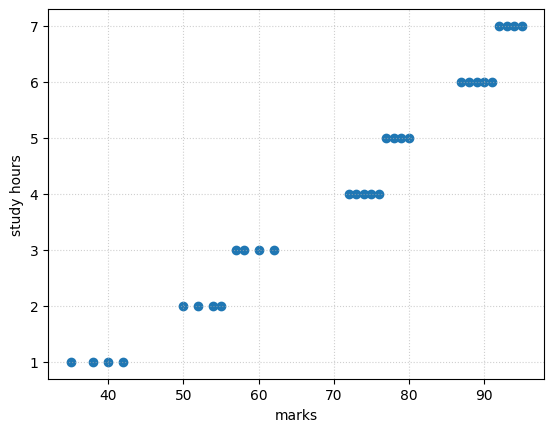
\includegraphics[width=0.75\textwidth]{img/exp7_markvsstudy.png}
    % \caption{Marks of Each Student — Bar Chart}
    % \label{fig:marks_bar}
\end{figure}

\subsubsection*{ii) Marks vs Attendance}

\begin{lstlisting}[style=python]
plt.scatter(df_student.Marks, df_student.Attendance)

plt.xlabel("marks")
plt.ylabel("attendance")
plt.grid(zorder = 0, linestyle = ':', alpha = 0.6)

plt.show()
\end{lstlisting}

\textbf{Output:}

\begin{figure}[H]
    % \centering
    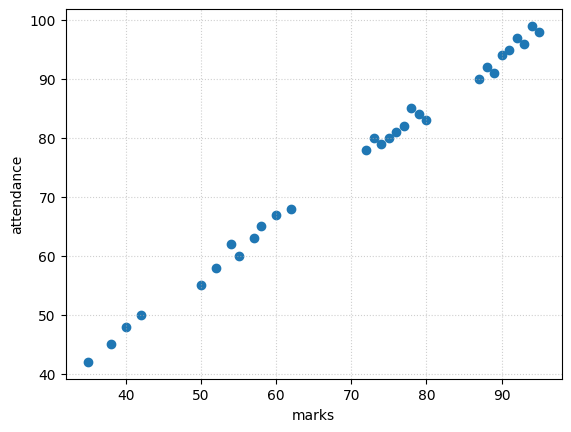
\includegraphics[width=0.75\textwidth]{img/exp7_markvsattend.png}
    % \caption{Marks of Each Student — Bar Chart}
    % \label{fig:marks_bar}
\end{figure}


\subsubsection*{iii) Attendance vs StudyHours}

\begin{lstlisting}[style=python]
plt.scatter(df_student.Attendance, df_student.StudyHours)

plt.xlabel("attendance")
plt.ylabel("StudyHour")
plt.grid(zorder = 0, linestyle = ':', alpha = 0.6)

plt.show()
\end{lstlisting}

\textbf{Output:}

\begin{figure}[H]
    % \centering
    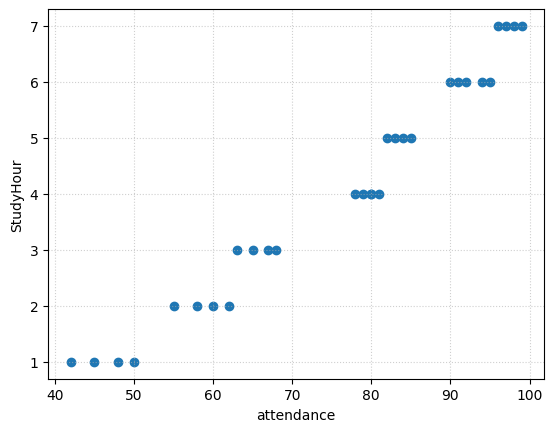
\includegraphics[width=0.75\textwidth]{img/exp7_attendvsstudy.png}
    % \caption{Marks of Each Student — Bar Chart}
    % \label{fig:marks_bar}
\end{figure}

\subsection{Observation}

i. All three scatter plot show a positive correlation. As one variable increases the other tends to increase as well.

ii. The Marks vs Attendance scatter plot shows the strongest positive correlation among all three pairs. Data points lie very close to a diagonal line, it's a near perfect relationship between them.

iii. Both the Marks vs StudyHours and StudyHours vs Attendance plots show stepeed \& cluseted pattern due to StudyHours being a discreate variable rather than continuous.

iv. No negative or zero correlation was observed in any pair.

v. The strong correlation in Marks vs Attendance plot suggest that attendance may be strong predictor of marks than StudyHours. 

